\documentclass[12 pt]{article}
\usepackage[a4paper, top=2.5cm, bottom=2.5cm, left=2.5cm, right=2.5cm]{geometry}
\pdfoutput=1 % if your are submitting a pdflatex (i.e. if you have % images in pdf, png or jpg format)
\usepackage{hyperref}
\usepackage{graphicx,color,rotating}

\def \aap  {A\&A}
\def \aaps  {A\&AS}
\def \aj  {AJ}
\def \apj  {ApJ}
\def \apjs  {ApJS}
\def \apjl  {ApJL}
\def \apss  {AP\&SS}
\def \araa  {ARA\&A}
\def \jcap  {JCAP}
\def \prd {Phy. Rev. D}
\def \ssr {SSRv}
\def \mnras {MNRAS}
\def \nat {Nature}
\def \physrep {Phys. Rept.}
\def \pasj {PASJ}
\def \etal {et~al.~}
\def \rmxaa {RMxAA}
\def \jgr {JGR}
\def \pasp {PASP}

\newcommand{\FIXME}[1]{{\color{red}{\em Comment: }{#1}}}

\usepackage[T1]{fontenc} % if needed
\usepackage{multicol}
\frenchspacing
\usepackage[para]{footmisc}

 
%\author{\vspace{-0.5cm}{\large \bf{Mattia Di Mauro}} (mdimauro@slac.stanford.edu)}
\date{}
%\date{\today}
% in alternativa a \date il comando \today introduce la data di sistema.


\begin{document}
%\maketitle

%\vspace{-1.0cm}
%\paragraph{Searching for a dark matter contribution to the extragalactic $\gamma$-ray background}

\vspace{-2.0cm}
\paragraph{Scientific rationale}
%Cosmic $\gamma$ rays are associated with the most extreme phenomena and sources and, not surprisingly, measurements in this part of the electromagnetic spectrum have triggered huge interest and are the goal of several current and future experiments. The {\it Fermi}-LAT
%\footnote{{\it Fermi}-LAT \url{https://fermi.gsfc.nasa.gov}, H.E.S.S. \url{https://www.mpi-hd.mpg.de/hfm/HESS/}, VERITAS \url{https://veritas.sao.arizona.edu}, HAWC \url{https://www.hawc-observatory.org} and CTA \url{https://www.cta-observatory.org}.} has revolutionized our understanding of the $\gamma$-ray sky at GeV energies while Imaging Atmospheric Cherenkov Telescopes (IACTs) (e.g., H.E.S.S., VERITAS and HAWC) cover the TeV band.\FIXME{I don't think you really need this for a GI panel.}
%The {\it Fermi} Large Area Telescope (LAT) detects since 2008 $\gamma$ rays in the energy range $E \in [0.1,1000]$ TeV and has revolutionized our understanding of the $\gamma$-ray sky at the GeV energies detecting thousands of sources \cite{2015ApJS..218...23A}. 

The {\it Fermi}-LAT has revolutionized our understanding of the $\gamma$-ray sky at GeV energies.
%while Imagining Atmospheric Cherenkov Telescopes (IACTs) (e.g., H.E.S.S., VERITAS and HAWC) cover the TeV band.
One of the greatest achievements of the {\it Fermi}-LAT is the precise measurement of the energy spectrum and the anisotropy of the so-called Isotropic Diffuse $\gamma$-Ray Background (IGRB) \cite{Ackermann:2014usa,2012PhRvD..85h3007A}. 
%The IGRB is a quasi-isotropic emission that is needed, together with the flux of detected sources and the Interstellar Emission (IE), to explain $\gamma$-ray data detected by the LAT.
The IGRB is a quasi-isotropic emission attributed to the combination of unresolved sources and a possible
truly diffuse background. It was first measured a few decades ago but its exact composition is still a mystery.
%The Extragalactic $\gamma$-ray background (EGB) is the sum of resolved extragalactic sources and

The bulk of the IGRB is likely the emission from unresolved, i.e. undetected, blazars that are the most numerous population of sources in {\it Fermi}-LAT catalogs (see, e.g., \cite{Ajello:2015mfa}).
Blazars are traditionally divided into BL Lacertae (BL Lacs) and Flat Spectrum Radio Quasars (FSRQs),
A sizable contribution could be due to misaligned Active Galactic Nuclei (MAGN). 
These sources are less luminous than blazars but, because they are much more numerous, the collective $\gamma$-ray emission could explain a significant part of the IGRB (see, e.g., \cite{DiMauro:2013xta}).
Finally, Star-Forming Galaxies (SFGs) produce $\gamma$ rays through the interaction of cosmic rays with the interstellar medium (see, e.g., \cite{2012ApJ...755..164A}).
%Considering the uncertainties, blazars, MAGN and SFGs contribute roughly with the same amount to the IGRB (see Fig.~\ref{fig:igrbcomp}).
%\FIXME{How much might they contribute, roughly?}
A fraction of the IGRB can originate from truly diffuse mechanisms such as the interaction of Dark Matter (DM) particles. Cosmology and Astrophysics provide convincing evidence that DM constitutes 26\% of the energy content of the Universe and detecting $\gamma$ rays produced from this elusive form of matter is one of the most promising strategies to search for DM.  
%Since the IGRB is derived with a subtraction from LAT data of all known $\gamma$-ray mechanisms, such as the interstellar emission and flux from cataloged sources, it is one of the most promising observable to search for a DM signature in $\gamma$ rays. \FIXME{I don't understand the logic in this last sentence.}

In Fig.~\ref{fig:igrbcomp} we show the contribution of each source population to the IGRB as derived in \cite{DiMauro:2015tfa}\footnote{Similar results have been found in \cite{Ajello:2015mfa}}.
The contribution of blazars, SFGs and MAGN to the IGRB integrated above 1 GeV is: $(39^{+15}_{-13})\%$, $(45^{+70}_{-30})\%$ and $(14^{+13}_{-7})\%$, respectively. 
Therefore, the fraction of the IGRB that is truly unresolved is between $0$ and $52\%$.
These large uncertainties reduce the sensitivity of searches targeting the DM contribution to the IGRB.
However, given the large size of the putative DM annihilation signal, improving significantly our knowledge for total contributions of these astrophysical components to the IGRB flux would make this particular probe highly competitive with other searches \cite{Charles:2016pgz}. 
%However, given the large size of the putative DM annihilation signal, knowing the fraction for the total contributions of these astrophysical components to the IGRB flux at the 10\% level would make this particular probe highly competitive with other searches \cite{Charles:2016pgz}. 
%The different source populations contribute with about the same flux to the IGRB at 1 GeV.
%The contribution of blazars, which are traditionally divided into BL Lacertae (BL Lacs) and Flat Spectrum Radio Quasars (FSRQs), has a relative uncertainty of about $30\%$ while the contributions of SFG and MAGN is known at $50\%$.
%The uncertainty levels that we quote in this proposal are relative to the average contribution of each source population.
%\FIXME{Is this relative or absolute?  I'd recommend giving the uncertainties in absolute terms if possible.}
%\FIXME{Do we have a reference for this claim?  Also, I think it would be clearer if we framed this in terms of the uncertainty on the  unaccounted for fraction of the IGRB.}
%We need to improve significantly the prediction of $\gamma$-ray emission from these sources at least to the 20\% level in order use the IGRB as a promising target for the detection of DM.  ``given the expected size of a putative DM annihilation signal, knowing the contributions of each of the astrophysical components at the 20\% level would allow up
%\FIXME{Can you give a rough estimate of how much?}


{\bf 
%I propose to use future {\it Fermi}-LAT catalogs, data and a multi-pronged approach to obtain the most precise determination of the contribution of extragalactic sources to the IGRB.  
We propose to use future {\it Fermi}-LAT catalogs, data and a multi-pronged approach to obtain a determination for the fraction of the contribution of extragalactic sources to the IGRB with a precision of 10\%.  
This result will improve our knowledge of the IGRB composition and will provide the space density and cosmological evolution of AGN and SFGs. 
%Moreover will enable us to find signatures or derive stringent limits for the DM production of $\gamma$ rays for candidates with an annihilation cross section  
Moreover, will enable us to find signatures or derive stringent limits for a DM contribution. 
Our analysis is conceived to detect DM particles with cross sections well below the thermal one for a wide range of DM masses.
We plan to release all results and tools that we are going to produce with this proposal. 
We believe that this would be an important service for the community that could use our products for their own analysis of {\it Fermi} data and to create the basis for analysis of data from future missions data such as Amego\footnote{\url{https://asd.gsfc.nasa.gov/amego/index.html}}, CTA \cite{Ong:2017ihp} and e-ASTROGAM \cite{Tatischeff:2016ykb}.}
%This will include updated list of $\gamma$-ray blazars, MAGN and SFGs, data for the flux of $\gamma$ rays for each source population, tools used to find the luminosity function from source catalogs, tools to derive source count distribution of extragalactic sources and to detect signatures or limits for a DM contribution. 
%The scientific community will benefit from the possibility to employ these products for their own analysis of {\it Fermi} data and to analyze future missions data such as CTA \cite{Ong:2017ihp}, e-ASTROGAM \cite{Tatischeff:2016ykb} or ComPair \cite{Moiseev:2015lva}.


\begin{figure} %  figure placement: here, top, bottom, or page
   \centering
  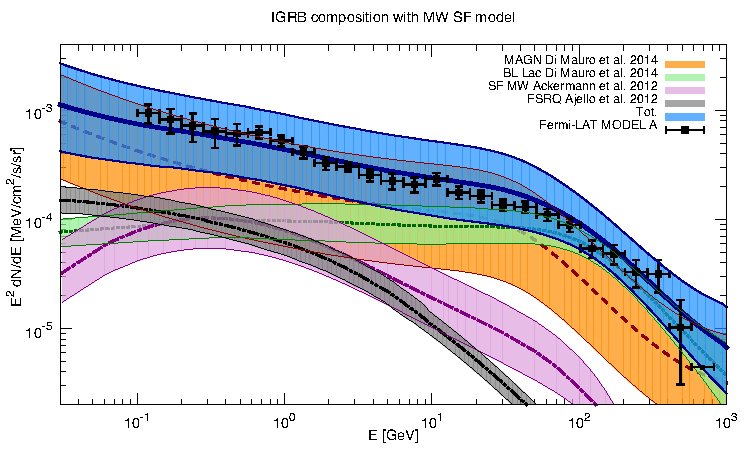
\includegraphics[width=4.0in]{fluxcompart_2014_unr.pdf} 
\vspace*{-4mm}
   \caption{$\gamma$-ray flux from unresolved sources, along with IGRB data \cite{Ackermann:2014usa}. Lines and relevant uncertainty bands represent the contribution from the following source populations: orange dashed for MAGN,  green dotted for BL Lacs, grey double dot-dashed for FSRQs, purple dot-dashed for SFG, and blue solid for the sum of all the contributions \cite{DiMauro:2015tfa}.}
   \label{fig:igrbcomp}
\end{figure}


\vspace{-0.5cm}
\paragraph{General methodology} 
\label{sec:methodology}
Below we list the different techniques we will planning to use in order to achieve our goals.  
%\FIXME{I'm still not really seeing the difference between the LF / SED and the efficiency corrections.  It seems to me like the efficiency corrections is just an improved version of the LF / SED.  What am I missing?}

{\it Luminosity function and SED of blazars.}
New catalogs of $\gamma$-ray sources will be available from the {\it Fermi}-LAT (see the preliminary version of the 4FGL\footnote{\url{https://fermi.gsfc.nasa.gov/ssc/data/access/lat/fl8y/}} with about 5600 sources).
%, almost a factor of two more sources than the 3FGL catalog).
We will use these catalogs to re-evaluate the luminosity function and cosmological evolution of blazars.
The luminosity function is the number density of sources as a function of redshift and $\gamma$-ray luminosity and it is the key ingredient for the estimation of $\gamma$-ray emission from blazars.
%It is usually parametrized with a Pure Luminosity Evolution (PLE) or Luminosity Dependent Density Evolution (LDDE) model  \cite{2012ApJ...751..108A}.
The luminosity function parameters are found by comparing, through a maximum-likelihood estimator, the numbers of expected objects to the observed number while accounting for selection effects in the survey \cite{2012ApJ...751..108A}. 

An important ingredient for the determination of $\gamma$-ray emission from blazars is the estimate of their Spectral Energy Distribution (SED).
We plan to use SED data from {\it Fermi}-LAT, ground-based $\gamma$-ray observatories (such as CTA, H.E.S.S., VERITAS and HAWC) and X-ray experiments (e.g. Swift, Chandra and NuSTAR) on individual sources to model their SEDs in a wide energy range.
This study will also result in estimates of the spectrum and cosmological evolution of the extragalactic background light that affects the propagation of very-high-energy $\gamma$ rays \cite{2012Sci...338.1190A}.

The current estimates for the luminosity function of blazars are based on the 1FGL and 2FGL catalogs (see, e.g., \cite{2012ApJ...751..108A,Ajello:2015mfa,DiMauro:2013zfa}).
The upcoming 4FGL will have about three times the number of sources as the 1FGL and 2FGL catalogs.
{\bf Using this more numerous sample of blazars we plan to find the blazar luminosity function and SED and we will be able to calculate the fraction for the contribution of these sources to the IGRB with a precision of 4\%.}

%I will select for this study blazars from the future 4FGL {\it Fermi}-LAT catalog that will be published in the middle of 2018. This analysis will bring to a publication that will include the calculation of the luminosity function and the contribution to the IGRB of BL Lacs and FSRQs. For the completion of this analysis about one year is needed: 6 months for the analysis and 6 months for the {\it Fermi}-LAT internal and journal review process.


{\it Efficiency corrections and photon statistics.}
%The method explained in the previous section relies on the {\it Fermi}-LAT detected sources and it is affected by extrapolation below the sensitivity of LAT catalogs. 
The luminosity function method is model-dependent in the sense that the functional form of the luminosity function is assumed based on model predictions.
Moreover, it relies on sources of {\it Fermi}-LAT catalogs. We plan to use two additional complementary techniques to find the contribution of blazars to the IGRB: efficiency corrections and photon statistics.
These methods do not depend on extrapolations, reach a sensitivity below the limits of the LAT catalogs and are model independent.
The drawback of these additional methods is that they cannot distinguish between different source populations since they derive the source count distribution of all sources in the extragalactic sky, which is dominated by blazars.
%Despite the fact that this analysis cannot separate individual components, it can provide the contribution of blazars to the EGB and IGRB, since {\it Fermi}-LAT catalogs are dominated by this source population. 

With the efficiency correction method, simulations of the $\gamma$-ray sky are generated to calculate the efficiency for detection of sources with a given photon flux $S$. 
The efficiency is then used to correct the source count distribution of cataloged sources and to find the real (i.e., intrinsic) $dN/dS$ of extragalactic sources~\cite{TheFermi-LAT:2015ykq}.
The efficiency correction method uses information down to the flux of the faintest source in the catalog while pixel photon count statistics reach even lower fluxes.
Specifically, the pixel photon count statistics method calculates the number of photons per pixel, and thus includes information from unresolved sources contributing even a single photon~\cite{TheFermi-LAT:2015ykq}.
%We have successfully used this method for the 2FHL catalog deriving that blazars contribute to the $86\%$ of the EGB above 50 GeV (see, e.g., \cite{TheFermi-LAT:2015ykq}). 



We plan to perform this analysis on at least 10 years of LAT data and in at least eight energy bins between 0.1-1000 GeV. This will enable us to evaluate more precisely than ever before the energy-dependence of blazar contribution to the IGRB.  That will, in turn, be a powerful tool to understand the SED of the source populations (SFGs or MAGN) and/or diffuse processes (e.g., DM particle interactions) that contribute to the IGRB along with blazars.

%The timescale for this analysis is one year since it needs to perform many simulations and analysis with {\it Fermi} Science Tools. 
%This analysis will be done in parallel to the determination of the luminosity function of blazars with the 4FGL catalog (see previous section).


%\begin{figure}[htbp] %  figure placement: here, top, bottom, or page
%   \centering
%  \includegraphics[width=2.8in]{1ppdf_2fhl.png} 
%\includegraphics[width=2.8in]{dNdS_2fhl.png} 
%   \caption{Left panel: Comparison between the pixel count distribution from the average of 20 simulations (blue points), %and the distribution from the real sky (red points). Right panel: intrinsic $S^2dN/dS$ distribution (black points). The black %solid line shows our best-fit model, while the grey and cyan bands show the $1\sigma$ and $3\sigma$ uncertainty bands %from the photon fluctuation analysis. The vertical brown dotted line represents the sensitivity of the photon fluctuation %analysis. The orange and red curves indicate where $85\%$ and $100\%$ of the EGB intensity above 50 GeV %\cite{TheFermi-LAT:2015ykq}. }
%   \label{fig:2fhldnds}
%\end{figure}






{\it Contribution of MAGN and SFGs to the IGRB: luminosity correlations.}
The majority of the uncertainty in the composition of the IGRB is due to SFGs and MAGN \cite{DiMauro:2015tfa} (see Fig.~\ref{fig:igrbcomp}). 
This is due to the limited sample of MAGN and SFGs detected in $\gamma$ rays and to the uncertain correlation between $\gamma$-ray and infrared or radio luminosities.
Indeed, the $\gamma$-ray luminosity function is estimated from measurements at these lower energies where the samples of SFGs and MAGN contain hundreds of sources \cite{2012ApJ...755..164A,DiMauro:2013xta}.


We plan to calculate the $\gamma$-ray emission of the SFG and MAGN source populations using future {\it Fermi}-LAT catalogs (e.g., 4FGL) that will include many more sources belonging to these source classes since SFGs and MAGN are on average faint $\gamma$-ray sources.
We will derive the correlation of $\gamma$-ray and radio (for MAGN) or infrared (for SFGs) luminosity using this more numerous than before sample of $\gamma$-ray sources.
For MAGN and SFGs that are not detected by {\it Fermi}-LAT we will calculate upper limits for their $\gamma$-ray luminosity.
We will combine the information derived for detected and undetected sources to reduce significantly the uncertainties in the correlation between $\gamma$-ray and radio or infrared luminosities which will allow a more precise estimate of the contribution of SFGs and MAGN to the IGRB.


%I plan to perform this analysis in the energy range 0.1-1000 GeV and to use for MAGN a collection of radio catalogs (e.g. 3CRR Bright Sample, The MRC 1 Jy Sample, The MS4 Sample and The BRL Sample, the FRICAT \cite{Capetti:2016srb} and FRIICAT \cite{Capetti:2017fjb}) and for SFGs infrared catalogs (e.g. \cite{Sanders:2003ms,2004ApJ...606..271G}).

%The $\gamma$-ray analysis will be executed with the {\it Fermi}-LAT Science tools. We expect a time scale of 6 months to complete this study and other 6 months for the {\it Fermi}-LAT internal and journal review process.



{\it Contribution of MAGN and SFGs to the IGRB: cross correlations.} 
We propose to study the contribution of MAGN and SFGs searching for cross correlations between IGRB photons and catalogs of extragalactic sources.
%This method, called cross-correlation technique, aims in finding correlations between the photons of the IGRB and the position of sources in catalog at low-energy (radio, optics and infrared).
Since SFGs and MAGN are faint sources and thousands of these objects have been detected in radio (for MAGN) and IR (for SFGs), if they contribute significantly to the IGRB they should leave an imprint in the IGRB.
This signature can be detected as correlations between IGRB photons and the position of these sources in low-energy catalogs.
This analysis has been successfully used in the past to find a correlation at $16.3\sigma$ significance between the IGRB and the NRAO VLA catalog (NVSS) of radio sources \cite{Cuoco:2017bpv}.
We plan to apply the cross-correlation analysis to at least 10 years of data and in at least 8 energy bins between 0.1 GeV to 1 TeV using the same method as in \cite{Cuoco:2017bpv}. We will mask the sources in the future 4FGL catalog, the Galactic plane and the regions such as the {\it Fermi} Bubble and Loop I that are known Galactic contributors. 
%We will use any future release by the {\it Fermi}-LAT team of improved models for the IE.
We will search for cross correlations between the IGRB and catalogs of SFGs and MAGN such as: 3CRR Bright Sample, the MRC 1 Jy Sample, the MS4 Sample and the BRL Sample, the FRICAT \cite{Capetti:2016srb} and FRIICAT \cite{Capetti:2017fjb}) for MAGN and \cite{Sanders:2003ms,2004ApJ...606..271G} for SFGs.
We will use the cross-correlation signal to find the $\gamma$-ray luminosity function for MAGN and SFGs starting from the one in radio and IR.
{\bf The results for the luminosity correlations derived from undetected and detected sources and for their luminosity function found with the cross-correlation analysis will be used to determine the fraction of the SFG and MAGN contribution to the IGRB at the 3\% and 9\% level, respectively.}

%{\it Stacking analysis of the $\gamma$-ray emission from MAGN and SFGs.} 
%MAGN and SFGs are on average faint $\gamma$-ray sources thus we expect that the sample of {\it Fermi}-LAT undetected  sources belonging to these source classes is very numerous. 
%We propose to apply a stacking analysis of the $\gamma$-ray emission from MAGN detected at radio energies and unresolved by {\it Fermi}-LAT. The stacking analysis for SFGs detected in infrared will be performed with an other proposal submitted in the {\it Fermi} GI cycle 11 (P.I. V.S. Paliya and Co.I. M. Ajello and M.Di Mauro).
%We will use the most-current radio and infrared catalogs of MAGN and SFGs. 
%%I will run a {\it Fermi}-LAT analysis for the detection of a point source for each target. 
%We will select only sources with a $TS<25$\footnote{The $TS$ is defined as twice the difference in log-likelihood between the null hypothesis (i.e., no source present) and the test hypothesis: $TS = 2 ( \log\mathcal{L}_{\rm test} - \log\mathcal{L}_{\rm null} )$.}. Point sources with a $TS>25$ are in fact included in LAT catalogs and are thus officially detected.
%We will run analysis searching for $\gamma$-ray emission from a point source with a given photon flux and index, stacking the photons from all sources in our sample. 
%This technique is able to detect the $\gamma$-ray emission from a population of faint point sources because even if each source contributes only a few photons the total emission from the entire sample will produce a significant flux.
%%As I explained before, the $\gamma$-ray emission from SFGs and MAGN is based on correlations between $\gamma$-ray and infrared (for SFGs) and radio (for MAGN) luminosities. 
%%I propose to divide the sample of undetected sources in bins of radio and infrared luminosities and to compute the stacking analysis to the sample of sources in each luminosity bin. 
%This stacking analysis will be applied to samples of sources binned in radio (for MAGN) or infrared luminosities (for SFGs) in order to calculate for each bin the detection or an upper limits for the $\gamma$-ray luminosity. 
%{\bf The results for the luminosity correlations derived from the stacking analysis of $\gamma$-ray undetected sources and for the list of numerous $\gamma$-ray detected sources will be used to reduce the uncertainty for the contribution of SFGs and MAGN to the IGRB to the 20\% level.}
%%This analysis will follow the same timescale of the previous one.


{\it Signatures or limits for the contribution of DM to the IGRB.}
The analyses described above will provide the most precise estimation of the contribution of extragalactic sources to the IGRB and they will permit us to search for DM signals in the IGRB with greatly improved sensitivity. 
%I plan to follow the same method employed in \cite{DiMauro:2015tfa,Ajello:2015mfa} to find signatures or derive limits for the contribution of DM to the EGB and IGRB.
N-body simulations predict that DM is distributed in the Universe with a main halo and substructures in each galaxy.
A possible contribution of $\gamma$ rays from DM is thus made of three components with distinct morphologies: a Milky Way smooth DM distribution, Milky Way substructures and an extragalactic component from other galaxies.
The extragalactic DM annihilation signal is isotropic to a large degree while the smooth Galactic and Galactic substructure components are more concentrated toward the center of our Galaxy.
We plan to include the contribution of each of these components following~\cite{Cirelli:2010xx,Ajello:2015mfa} and any upcoming N-body simulation results.

In our analysis we will first perform a fit to {\it Fermi}-LAT IGRB data optimizing the parameters that affect the $\gamma$-ray emission of AGN and SFGs. 
%At a first approximation I will just use the normalization and the slope of source SEDs for each source population.
%This analysis will provide the goodness of fit for the null hypothesis for which the IGRB and EGB are explained with astrophysical sources. 
Then, we will add the $\gamma$-ray emission from Galactic and extragalactic DM (see, e.g, \cite{DiMauro:2015tfa,Ajello:2015mfa}). For a fixed DM mass ($M_{\rm{DM}}$), we will add as a free parameter in the fit the annihilation cross section of DM ($\langle \sigma v \rangle$).
%, in addition to the ones for astrophysical sources.
The goodness of fit from this analysis is compared to the one with astrophysical sources only will provide the significance for the contribution of DM.
We will perform this analysis for different DM annihilation and decay channels and for DM masses between the energy threshold of the DM candidate and 10 TeV.
The result of this analysis will be either the signature of a DM contribution, if the fit to {\it Fermi}-LAT data improves significantly with the addition of this component, or will provide upper limits for $\langle \sigma v \rangle$ as a function of the DM mass and annihilation or decay channel.

%This analysis will be performed after the ones explained in previous sections during the third year of my project.



\vspace{-0.5cm}
\paragraph{Feasibility of the project}
{\it Contribution of blazars to the IGRB and limits for DM.}
Forecasts for the contribution of extragalactic sources to the IGRB and for the limits on a DM contribution with 15 years of LAT operations have been published in \cite{Charles:2016pgz}.
We have shown that with future {\it Fermi}-LAT catalogs we will be able to reduce by 30-50\% the uncertainty of the contribution of extragalactic sources to the IGRB (see left panel of Fig.~G.33).
We have also calculated that with a significant improvement in the modeling of the IE we will be able to reduce the systematic uncertainties of the IGRB and we will be able to find limits for DM that rule out the thermal cross section up to 200 GeV.
These limits will be as good as the stacking analysis of clusters or of Milky Way Dwarf Spheroidal Galaxies \cite{Charles:2016pgz}. 
%\FIXME{Do we have a reference here.}

%Using the intrinsic source count distribution of blazars of the 1FGL catalog \cite{2010ApJ...720..435A} and modeling the SED of the individual blazars with single power laws, the predicted number of detected blazars with 15 years of data is about 3300.
%This number compared to the number of blazars in the 3FGL has been used to rescale the uncertainty for the contribution of blazars to the EGB.
%The same procedure has been used also to estimate the uncertainty for the MAGN contribution to the EGB considering 70 MAGN detectable in 15 years. See left panel of Fig.~G.33 of \cite{Charles:2016pgz} for the forecast of the contribution of extragalactic sources to the EGB in 15 years of {\it Fermi}.
%In Fig.~\ref{fig:igrb15years} I show the contribution from MAGN, blazars and SFGs calculated with the method explained above.
%We used in \cite{Charles:2016pgz} this estimate to calculate the limits for the annihilation cross section of DM particles.



%\begin{figure}[htbp] %  figure placement: here, top, bottom, or page
%\centering
%\includegraphics[width=4.0in]{sourcesegb_15years.png} 
%\caption{Contribution of blazars (cyan band), MAGN (green band) and SFGs (gray band) to the {\it Fermi}-LAT EGB data %(black points). The total best fit of the summed contributions from AGN (blazars and MAGN) and SFG is depicted with a %solid red line, with the orange uncertainties given by the orange band \cite{Charles:2016pgz}. }
%\label{fig:igrb15years}
%\end{figure}


{\it Contribution of MAGN to the IGRB.}
As explained before, one of the greatest sources of uncertainty for the interpretation of the IGRB is the contribution of MAGN and in order to reduce it we need a large sample of such sources in future {\it Fermi} catalogs.
We investigated this considering these radio catalogs of MAGN: 3CRR Bright Sample, the MRC 1 Jy Sample, the MS4 Sample and the BRL Sample, the FRICAT \cite{Capetti:2016srb} and FRIICAT \cite{Capetti:2017fjb}).
We eliminated from these catalogs sources that also appear in the blazar catalog BZCAT \cite{Massaro:2015nia} or in SFG catalogs \cite{Sanders:2003ms,2004ApJ...606..271G}. 
We have then performed a dedicated $\gamma$-ray analysis with the {\it Fermi} Science Tools in the energy range 0.1-1000 GeV and for 100 months of data. 
The result of this analysis is that we find a sample of 46 MAGN, more than twice the sample detected in the 3FGL, demonstrating the viability of our proposal.

%In Fig.~\ref{fig:magn} we show the $\gamma$-ray luminosity and photon index for the new MAGN and for radio galaxies, %SSRQs and blazars detected in the 3FGL. MAGN are fainter than blazars because of the jet that is misaligned with respect to the line of sight and have softer SEDs. This is clear looking to the position of radio galaxies, SSRQs (that are both MAGN) detected in the 3FGL and MAGN in our analysis that on average populate the top right plane while blazars are located in the opposite part. 
%This demonstrates that the LAT detects many more MAGN with respect to the 3FGL and thus our plan of reducing the uncertainty for the contribution to the IGRB will be achievable.

%\begin{figure}[htbp] %  figure placement: here, top, bottom, or page
%   \centering
%  \includegraphics[width=3.0in]{Lgamma_index_3LAC_cand.pdf} 
%   \caption{$\gamma$-ray luminosity and photon index for blazars in the 3FGL (black point), 3FGL radio galaxies (red %stars), steep spectrum radio quasars (blue star) and new MAGN (green star).}
%   \label{fig:magn}
%\end{figure}


%{\it Contribution of SFGs to the EGB.}
%SFGs are very numerous in infrared catalogs but are on average faint $\gamma$-ray sources. 
%We tested this scenario and the feasibility of a stacking analysis of a faint population of sources taking the list of 64 SFGs reported in Tab.~1 of \cite{2012ApJ...755..164A}.
%We performed, with the collaboration of Dr.~V.~Palyia, a stacking analysis on these sources using 100 months of data in the energy range 0.1-1000 GeV finding a $TS=35$ with a best fit photon index of 1.8 and with an average flux per source of $6\times 10^{-11}$ ph cm$^{-2}$ s$^{-1}$.
%A test source with the same index and flux is placed at the position of each SFG and the {\it Fermi} Science tools for the detection of a point sources are ran on them stacking all the photons from each source.
%The result of this analysis is that we find a $TS=35$ for the stacked $\gamma$-ray emission of this sample of SFGs with a best fit photon index of 1.8 and with an average flux per source of $6\times 10^{-11}$ ph cm$^{-2}$ s$^{-1}$.
%We thus found a significant $\gamma$-ray emission (at more than $5\sigma$ significance) from our sample of SFGs. %We plan to perform this analysis with a much more numerous sample of SFGs (using \cite{Sanders:2003ms,2004ApJ...606..271G}) enabling to reach our goals.




{\it Source count distribution of blazars derived with efficiency correction and photon statistics.}
We performed in \cite{DiMauro:2017ing} an analysis of the source count distribution of blazars derived with efficiency corrections and photon statistics methods (1pPDF) using the third {\it Fermi} catalog of hard sources (3FHL) detected at $E>10$ GeV \cite{TheFermi-LAT:2017pvy}. We selected sources located at Galactic latitude $|b|>20^{\circ}$.
The efficiency correction and photon statistics methods give compatible results and they allow determination of the $dN/dS$ for almost three orders of magnitude. The sensitivity of the two methods is $\sim 10^{-11}$ ph cm$^{-2}$ s$^{-1}$ and summing the flux of cataloged sources and the contribution of unresolved sources we find that $(42\pm8)\%$ of the IGRB is explained with blazars.
%\FIXME{I think that the uncertainty on this number is very important.  Do you have it?  Also, are the number right, it looks like you have 42 +48 = 100, which isn't right?  Is there something else?}
%In the 3FHL and at $|b|>20^{\circ}$, $89\%$ of the detected sources are blazars meaning that this source population contributes only for a fraction of the EGB at these energies.
This result has remarkable consequences because the remaining $58\%$ of the IGRB should be given by an unresolved population of faint sources such as SFGs and/or MAGN or from a truly diffuse emission mechanism like DM particle interactions. 


{\it Example of a detectable DM contribution to the IGRB.}
We consider the average $\gamma$-ray emission from blazars, SFGs and MAGN as in Fig.~\ref{fig:igrbcomp} with an uncertainty of each contribution as reported in the goals of this proposal. We thus fix the uncertainty for the fraction of the blazar, SFG and MAGN contribution to the IGRB at $4\%$, $3\%$ and $9\%$, respectively.
We then add the contribution of extragalactic DM annihilating into $b\bar{b}$ with $M_{\rm{DM}}=100$ GeV and $\langle \sigma v \rangle = 10^{-26}$ cm$^3$/s for a model provided in \cite{Cirelli:2010xx}. 
{\bf This candidate has a cross section that is a factor of 2 below the thermal cross section and would contribute $25\%$ of the IGRB above 1~GeV.}
The result is shown in Fig.~\ref{fig:moneyplot}. The IGRB data points are mock data created by rescaling the errors of the published ones \cite{Ackermann:2014usa} by a factor of the square root of time for 10 years of data. The data have been renormalized by a factor of 0.83 due to the greater flux resolved by point sources in the preliminary 4FGL with respect to the 3FGL.
{\bf It is clearly visible from this example that with this proposal we will be able to detect the $\gamma$-ray emission from a DM candidate that is compatible with current DM bounds (see, e.g., \cite{Fermi-LAT:2016uux}).} Here we are reporting only the contribution of extragalactic DM from the main halo of Galaxies. Adding the Galactic main halo and substructures the signal would be even larger.



%\begin{figure} %  figure placement: here, top, bottom, or page
%  \centering
%  \includegraphics[width=3.0in]{limitsigrb_15years} 
%  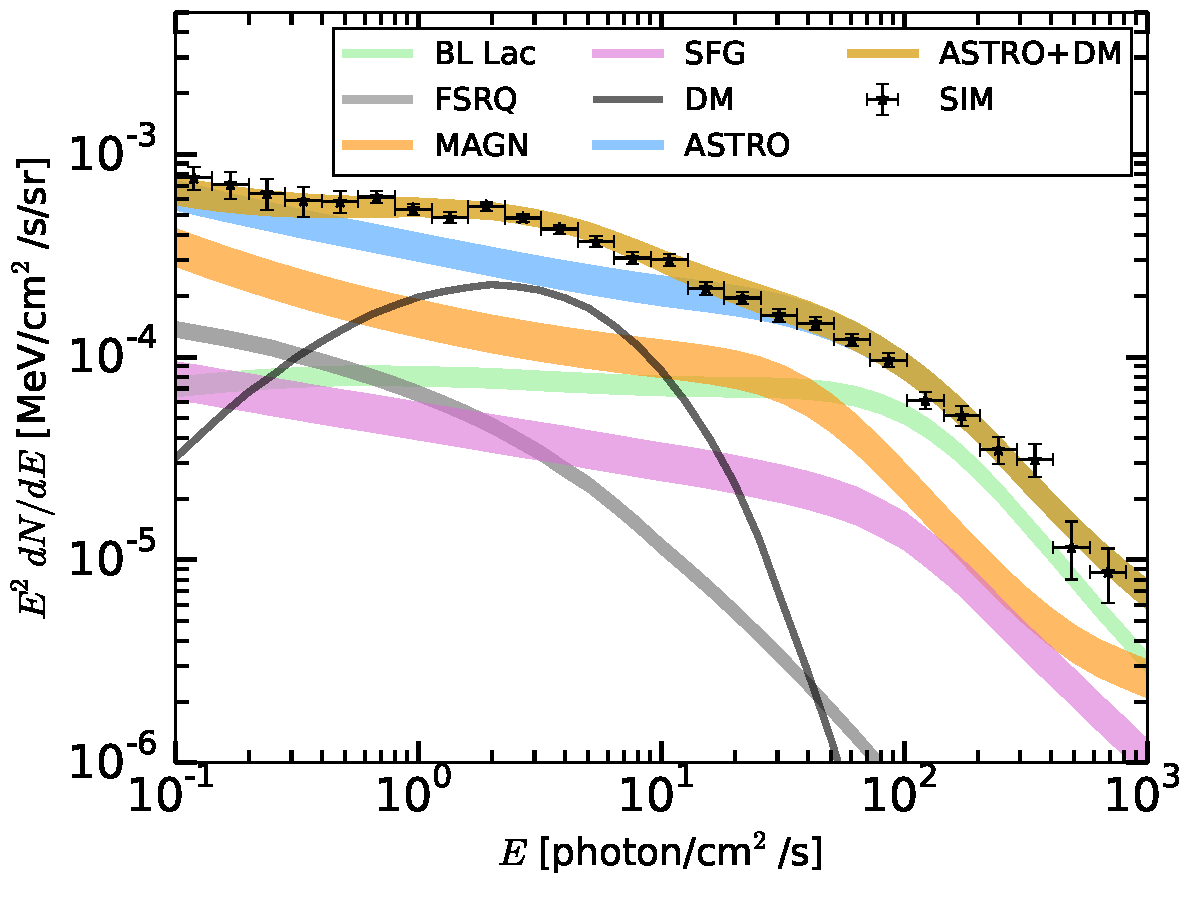
\includegraphics[width=3.0in]{money_plot_proposal.pdf} 
%   \caption{Left Panel: Projected upper limits on the WIMP annihilation cross section derived from the IGRB energy %spectrum after 15 years of data taking, compared to the limits derived in \cite{Ajello:2015mfa} (thin black solid line). %The dashed blue and red dotted curves correspond to cases in which the systematic uncertainties are reduced by %factors of 2 and 10, respectively, relative to their values in the 50-month analysis. In both cases, the statistical %uncertainties have been reduced by a factor of 2. The shaded red area corresponds to the uncertainties from the %modeling of the cosmological DM annihilation signal \cite{Charles:2016pgz}. 
%Right panel: Comparison of projected LAT limits for 15 years of data for the search methods described in %\cite{Charles:2016pgz}. }
%   \label{fig:igrblimits}
%\end{figure}

\begin{figure} %  figure placement: here, top, bottom, or page
 \centering
  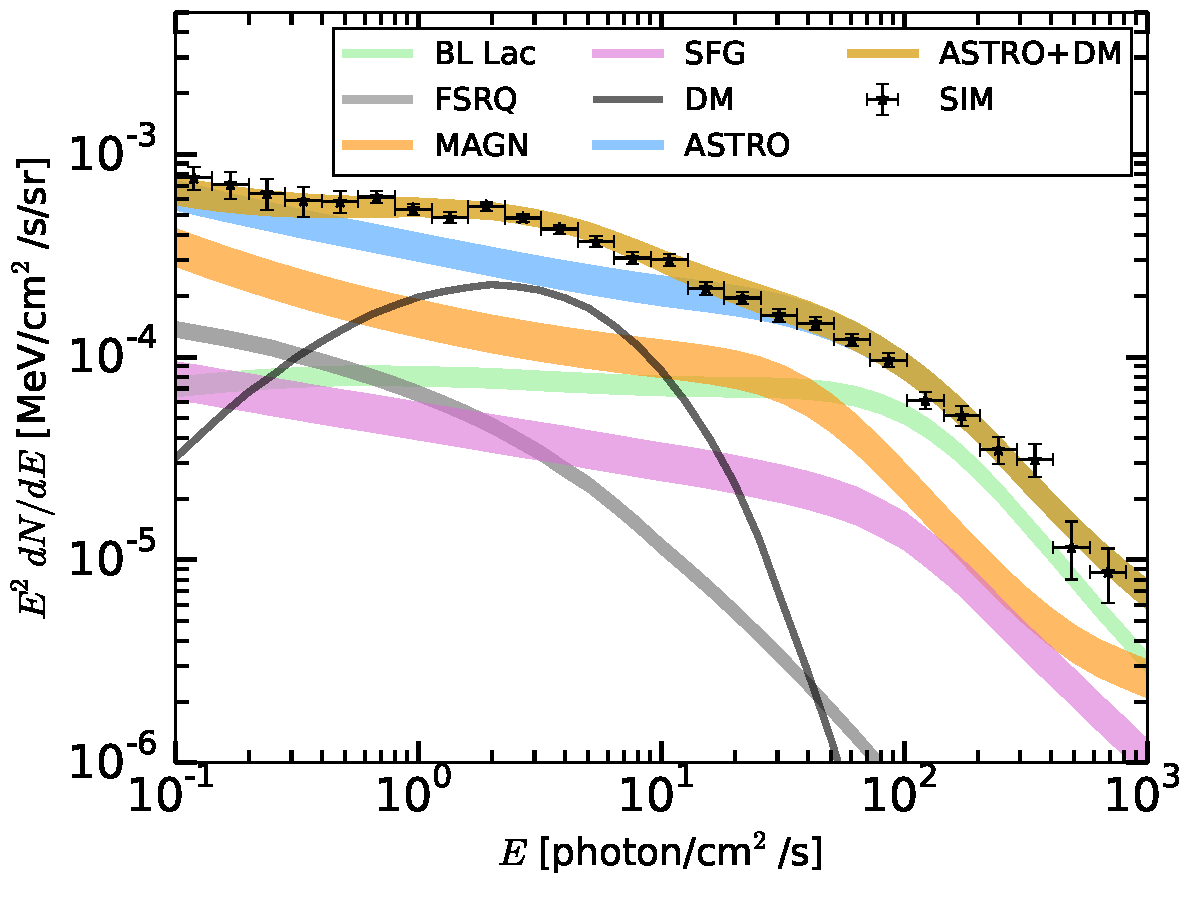
\includegraphics[width=3.5in]{money_plot_proposal.pdf} 
\vspace{-0.7cm}
   \caption{$\gamma$-ray emission from FSRQs, BL Lacs, MAGN, SFGs, as in Fig.~\ref{fig:igrbcomp} but with an uncertainties for the fraction of their contribution to the IGRB that is 4\% for blazars, 3\% for SFGs and 9\% for MAGN. A contribution from extragalactic DM annihilating into $b\bar{b}$ with $M_{\rm{DM}}=100$ GeV and $\langle \sigma v \rangle = 10^{-26}$ cm$^3$/s. The sum of the source population contributions and the DM annihilation signal is depicted as the gold band.}
   \label{fig:moneyplot}
\end{figure}


%\begin{figure}%  figure placement: here, top, bottom, or page
%   \centering
%  \includegraphics[width=3.5in]{dNdS_3FHL_pred_proporal_ldde.pdf} 
%   \caption{$dN/dS$ obtained with the efficiency correction method found for sources detected with $TS > 16$ (black %diamonds) and 25 (red stars). The $1\sigma$ statistical uncertainty band (brown band) for the result obtained with the %1pPDF method is reported. The additional light orange band depicts an estimate of systematic uncertainties using %different IEMs. The prediction from blazars with the LDDE luminosity function is shown with a cyan band %\cite{Ajello:2015mfa}.}
%   \label{fig:eff1ppdf}
%\end{figure}


\vspace{-0.5cm}
\paragraph{Data and Tools provided for the community.}
Our proposal involves the creation of a large amount of data and tools that we will release to the public. We plan to incorporate the tools to the {\tt FermiPy} Python package\footnote{\url{http://fermipy.readthedocs.io/en/latest/}} and we will upload the data to its GitHub repository and into the FSSC.
These products will include:
\begin{itemize}
\vspace{-0.3cm}
\item The list of blazars, SFGs and MAGN that we will use for our analysis.
We plan to keep our list periodically updated with newly found redshift measurements, with the most up-to-date SEDs, classification (FRI or FRII for MAGN, FSRQ or BL Lacs for blazars) and with infrared or radio luminosities.
\vspace{-0.3cm}
\item The measurements for the $\gamma$-ray anisotropy and flux generated by SFGs, MAGN and blazars. We will update these estimates when new {\it Fermi}-LAT catalogs are released or cataloged sources are newly associated with these source classes.
\vspace{-0.3cm}
\item The source count distribution at different fluxes and in energy bins calculated with efficiency correction and 1PDF methods.
\vspace{-0.3cm}
\end{itemize}
We will provide all the codes that we will employ in our projects with dedicated documentation including: evaluation of the luminosity function of blazars, simulation and analysis of $\gamma$-ray data, evaluation of detection efficiency and source count distribution for blazars, tools to calculate the $\gamma$-ray emission from DM.
{\bf The community will benefit in the near term and long term from using our products to make their own analyses of new {\it Fermi}-LAT data and of data from future $\gamma$-ray experiments such as Amego, CTA and e-ASTROGAM.}
%\FIXME{I think it would be good to be very explicit here and have an enumerated list of the deliverables.}

\vspace{-0.5cm}
\paragraph{Summary, Timeline of the Project and Budget}
The composition of the IGRB is an open problem in astrophysics.   
We will undertake deep searches for a signature of a DM contribution over the next two years.
%We plan to use future data from {\it Fermi}-LAT to tackle it from different directions.
{\bf The first year} will be devoted to the calculation of the luminosity function of blazars using the 4FGL, and to the determination of their source count distribution applying the efficiency correction and photon statistics methods to at least 10 years of {\it Fermi}-LAT data.  
This research will produce an estimate for the fraction of blazar contribution to the IGRB at the 4\% level.
{\bf In the second year} we will reduce to 3\% and 9\% level the uncertainties associated to the fraction of the SFG and MAGN contribution to the IGRB. This will be achieved using new {\it Fermi}-LAT catalogs and employing a cross correlation-study between the IGRB and SFGs and MAGN catalogs.
%This will be achieved using new {\it Fermi}-LAT catalogs and employing a stacking analysis of $\gamma$-ray undetected sources.
%We will take the results of the stacking analysis of SFGs derived with an other program proposed at this cycle of the {\it Fermi} GI (P.I. V.S. Paliya and Co.I. M. Ajello and M.Di Mauro).  
%\FIXME{What happens if that other proposal isn't selected?   Don't introduce something new in the summary.}
The work performed in this proposal will enable the most precise ever estimation of the contribution of extragalactic sources to the IGRB and will permit us to search for a signature or bounds for DM production of $\gamma$ rays.

Given the substantial data analysis effort, we request two years funding to support for the PI ($\sim 50\%$), for two conferences per year and publication charges. Including overheads we request a budget of 120k\$ per year. 
%\FIXME{Is that total, or per year?} 
The PI M. Di Mauro and CO-Is M. Ajello, V. Paliya, S. Manconi and H. Zechlin will be directly in charge of the analysis.%\FIXME{If you can make the space, list what parts of the analysis people will work on.}   
Co-Is E. Charles, F. Donato and S. Digel will provide both technical and the scientific input.



\vspace{-0.2cm}
{\footnotesize
\begin{multicols}{2}
\bibliographystyle{ieeetr}
\bibliography{Einstein.bib}
\end{multicols}}





\end{document}  

%  LocalWords:  blazars Lacertae blazar
